\documentclass[conference]{../cls/IEEEtran}

\usepackage{graphicx}

\begin{document}

\title{Early Estimation of Multi-Objective Traffic Behavior}

\author{
	\IEEEauthorblockN{Dominik Ascher}
	\IEEEauthorblockA{
		Chair IV: Software \& Systems Engineering\\
		Technische Universit\"at M\"unchen\\
		Boltzmannstr.\ 3, 85748 Garching, Germany\\
		Email: ds.ascher@gmail.com
	}
	\and
	\IEEEauthorblockN{Georg Hackenberg}
	\IEEEauthorblockA{
		Chair IV: Software \& Systems Engineering\\
		Technische Universit\"at M\"unchen\\
		Boltzmannstr.\ 3, 85748 Garching, Germany\\
		Email: hackenbe@in.tum.de
	}
}

\maketitle

\begin{abstract}
Intelligent Transportation Systems (ITS) have come a long way targeting recent problems of increasing emissions and growing vehicle numbers. Current approaches address a variety of objectives including congestion management, collision avoidance, energy-efficiency and emission reduction. However, respective solutions typically are designed for and tailored to a fixed subset of objectives. Consequently, the effects of changing objectives and priorities cannot be assessed easily. To overcome this situation we present a lightweight approach to estimating traffic behavior early in the systems engineering process using discrete-time and continuous-state system models. We then demonstrate the feasibility of the framework using a basic traffic scenario before concluding with an initial discussion and outlook.
\end{abstract}

\begin{IEEEkeywords}
Feasibility study, urban traffic control, eco-routing.
\end{IEEEkeywords}

\section{Motivation}

In recent decades, efforts to engineer ITS have come a long way, targeting contemporary and future problems of increasing emissions and growing vehicle numbers. Among the approaches two main directions can be distinguished: (1) Urban Traffic Control (UTC) focusing on multiple traffic participants and their interaction~\cite{Chen2010,Dresner2008} and (2) Eco-Routing focusing on a single traffic participant and his route~\cite{Ericsson2006, Barth2007,Boriboonsomsin2012}. In particular, UTC typically targets congestion management and collision avoidance~\cite{Chen2010}. Technically, the approaches rely on agent based techniques to describe human driving behavior with respect to traffic supervision and control~\cite{Chen2010}. More advanced approaches even consider fully autonomous vehicles thereby proposing an alternative to human-oriented traffic supervision and control~\cite{Dresner2008}. In contrast, Eco-Routing typically targets energy-efficiency and emission reduction~\cite{Ericsson2006,Barth2007}. Technically, the approaches rely on optimization techniques to describe route variables, constraints and objectives~\cite{Ericsson2006,Barth2007}. As frequent use of energy-efficient routes might cause congestion, advanced approaches finally incorporate historical and real-time traffic information thereby taking first steps towards bridging the gab between Eco-Routing and UTC~\cite{Boriboonsomsin2012}.

However, while the reviewed approaches offer feasible solutions towards specific objectives, they do not enable to balance and analyze multiple objectives and their resulting behavior in traffic systems. To overcome this situation, in this paper, we report on the first steps towards an operational feasibility study on multiple objective control strategies in traffic systems. We shortly describe the underlying behavior estimation framework before explaining the multiple objective control demonstrator as well as initial performance analysis results.

\subsection{Scope}

According to Whitten et al.~\cite{Whitten2005} in systems engineering feasibility studies follow the requirements discovery phase to uncover potential opportunities and threads. Upon successful feasibility demonstration the system design, implementation and operation phases follow.

\subsection{Contribution}

Technically, we base our work on early emergent property estimation techniques described in~\cite{Hackenberg2012}. Consequently, we use a discrete-time and continuous-state system model. We rely on discrete-time models to reduce the reachable state space during behavior estimation. However, we work with continuous-state models because quantities like velocity or distance can be described more intuitively. Moreover, we rely on a generic and reusable model architecture dividing the system into software, context, constraint, objective and equivalence components. In particular, the partial software model describes the control spectrum, while the context model describes the physical state. Based on the physical state the constraint and objective models define the operational limits and goals. Finally, the equivalence model describes how the physical states can be clustered during state space exploration. Behavior estimation uses stochastic optimization techniques similar to~\cite{Pereira1991} to approximate optimal system behavior.

\section{Energy-Efficient Urban Traffic Control}

Based on the aforementioned models and their related architecture, our approach
is consisted of individual vehicles according components and their individual
behavior. Simulation steps in our approach are measured in discrete time
intervals of 5 minutes. The behavior of the vehicle control component is
essentially defined by speed and edge selection. Edge selection is based on the available
choices on the current position of the observed vehicle. If a vehicle has
completely crossed an edge, it is able to select a new edge to travel to. Speed
selection depicts an average value for the time segment and depends on a
continuous average value range. The vehicle context component's behavior is defined by
relative position on the edge, charge state and vehicle energy consumption. A simplified approach towards energy
consumption estimation is employed: Energy consumption within a given time
segment is approximately determined via the current edge's altitude difference 
and average speed. Vehicle speed has a quadratic relationship to observed
energy consumption. In the equivalence component, the vehicles current speed is defined
for clustering during state space exploration. The vehicle objective component,
determines the operational goals and vehicle driving behavior in the traffic
system. Respective objectives are formulated as cost functions, which can
differently weighted in respect to each other. Cost function A measures the
elapsed time since the start of the simulation until reaching the target. Cost function B determines the vehicles current
energy consumption in relation to the vehicles maximum possible energy consumption.
Furthermore, in the traffic system objective component, different priorities of
vehicles in the traffic system can be introduced through weighting of their individual costs.
Finally, in the vehicle constraint component, a constraint tests, whether the
current charge state lies within minimum and maximum limits. Moreover, in the traffic
system constraint component, a collision constraint tests for every possible
pair of vehicles whether the sum of their currently selected relative position
on the edge and the vehicles length overlap and whether there are free lanes
available on the current position based on edge capacity.

For behavior estimation, we demonstrate a basic case of a
single vehicle within a traffic system with two energetically and
distance different routes. Both routes have the same starting points and target
destinations. While route A represents a longer, flat route, route B depicts a
shorter route with differing heights. According simulation results for speed selection and energy consumption over time are depicted in Figure 2 (Top). In a second case, we
compare how well our control approach copes with a multitude of vehicles and a larger traffic network with energetically different route profiles. In Figure 2 (bottom), the 
results to the evolution of speed selection and energy consumption for the
second case are depicted.

\begin{figure}[t!]
	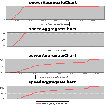
\includegraphics[width=\columnwidth]{../gfx/placeholder.pdf}
	\caption{Top: Comparison of the different control objectives in Case A. Bottom:
	Comparison of control objectives in Case B.}
	\label{figure:results}
\end{figure}


\section{Conclusion and Outlook}

We presented first steps towards studying the feasibility of a balancing
approach of multiple control objectives for urban traffic systems.
Preliminary behavior estimation results of driving behavior have been obtained and provided insight 
in possible trade-off considerations between multiple control objectives.
Further research has to show the feasibility of the approach towards a larger
problem size, more specific objectives and their respective balancing.

\bibliographystyle{../bst/IEEEtran}
\bibliography{ICCVE-2014}

\end{document}
